\documentclass[conference]{IEEEtran}
\IEEEoverridecommandlockouts

\usepackage{cite}
\usepackage{amsmath,amssymb,amsfonts}
\usepackage{graphicx}
\usepackage{textcomp}
\usepackage{xcolor}
\usepackage{booktabs}
\usepackage{array}

\newcommand{\SegTrain}{898}
\newcommand{\SegVal}{98}
\newcommand{\SegTest}{99}
\newcommand{\SegTotal}{1095}
\newcommand{\ClsTrain}{8055}
\newcommand{\ClsVal}{895}
\newcommand{\ClsTest}{1921}
\newcommand{\ClsTotal}{10871}
\newcommand{\SegIoU}{76.58}
\newcommand{\SegDice}{83.20}
\newcommand{\SegPrecision}{82.88}
\newcommand{\SegRecall}{85.82}
\newcommand{\SegMapFifty}{58.08}
\newcommand{\SegMapNinetyFive}{40.66}
\newcommand{\ClsAcc}{92.66}
\newcommand{\ClsMacroP}{92.87}
\newcommand{\ClsMacroR}{92.68}
\newcommand{\ClsMacroF}{92.63}

\def\BibTeX{{\rm B\kern-.05em{\sc i\kern-.025em b}\kern-.08em
    T\kern-.1667em\lower.7ex\hbox{E}\kern-.125emX}}

\begin{document}

\title{A Panel-Aware Lightweight Framework for Photovoltaic Panel Contamination Severity Mapping Under Complex Illumination}

\author{
\IEEEauthorblockN{Author Information To Be Completed Before Submission}
\IEEEauthorblockA{Replace this block with the final author list, affiliations, emails, and funding note if required}
}

\maketitle

\begin{abstract}
RGB inspection of photovoltaic (PV) panels is attractive for routine maintenance, but strong reflection, cast shadow, and background clutter make contamination analysis unstable in realistic outdoor scenes. This paper presents a panel-aware lightweight framework that first segments PV surfaces with a YOLOv8 branch and then performs tile-level severity classification to build per-panel contamination maps and pie-chart statistics. On a self-built dataset containing \SegTotal{} mask-labeled panel images and \ClsTotal{} severity tiles, the current reproducible baselines achieve \SegIoU{}\% IoU and \SegDice{}\% Dice for panel segmentation, and \ClsAcc{}\% top-1 accuracy with \ClsMacroF{}\% Macro-F1 for severity classification. These results show that a panel-localization prior can provide interpretable panel-level severity analysis and is a practical direction for lightweight PV inspection deployment.
\end{abstract}

\begin{IEEEkeywords}
photovoltaic inspection, contamination severity mapping, panel segmentation, image classification, image processing, complex illumination
\end{IEEEkeywords}

\section{Introduction}
Photovoltaic power plants operate in open outdoor environments and are therefore affected by dust accumulation, surface contamination, and local structural degradation. These factors reduce energy conversion efficiency and increase maintenance burden. Compared with manual patrol, RGB-image inspection is cheaper and easier to deploy at scale, but it is also more sensitive to strong reflection, cast shadow, viewpoint variation, and mixed background clutter \cite{ref_review,ref_rgbsoiling,ref_uavfault}.

For a short regular paper, the technical line must be frozen early. Based on the currently available annotated data, this work does not formulate the task as multi-defect detection with bounding boxes. Instead, it focuses on a more honest and better supported direction: panel-aware contamination severity mapping. The pipeline first extracts panel surfaces and then classifies small panel tiles into three severity levels, finally aggregating them into per-panel statistics. This definition keeps the task clear, matches the available labels, and still provides interpretable maintenance cues.

The contributions of this draft are summarized as follows.
\begin{itemize}
\item A panel-aware visual inspection framework is defined for PV contamination severity mapping under complex illumination. Its core idea is to use panel localization as a prior before severity analysis.
\item A complete dataset definition is provided for both stages: a panel segmentation dataset with \SegTrain/\SegVal/\SegTest{} train/validation/test images and a severity classification dataset with \ClsTrain/\ClsVal/\ClsTest{} train/validation/test tiles.
\item Reproducible stage-wise baselines are reported using real experiments, together with confusion analysis and representative failure modes that can support a stronger camera-ready comparison later.
\end{itemize}

\section{Related Work}
\subsection{PV Visual Inspection}
Recent PV inspection studies span infrared diagnosis, electroluminescence imaging, and RGB-based soiling analysis \cite{ref_review,ref_uavfault}. RGB inspection remains attractive because it has low hardware cost and directly captures visible contamination. Cavieres \textit{et al.} used RGB images for soiling and partial shading assessment \cite{ref_rgbsoiling}, while Evstatiev \textit{et al.} studied visible-spectrum soiling recognition with machine learning \cite{ref_vissoiling}. However, many existing methods either stay at image-level classification or do not explicitly isolate PV surfaces before analysis.

\subsection{Panel Localization in Aerial or Outdoor PV Scenes}
Panel localization quality strongly affects downstream analysis. Arnaudo \textit{et al.} compared deep learning methods for PV panel detection in aerial scenes and showed that scene complexity and target scale materially influence performance \cite{ref_aerial}. Their findings support our choice to treat panel segmentation as an intermediate image-processing step rather than applying a classifier directly to the full image.

\subsection{Severity Analysis and Lightweight Deployment}
DeepSolarEye showed that soiling analysis benefits from spatially structured learning rather than pure image-level recognition \cite{ref_deepsolareye}. This idea is closely related to our use of panel-aware tiles. In lightweight deployment settings, the challenge is to preserve interpretability while keeping the pipeline simple enough for practical inference. The present draft therefore emphasizes a single main improvement point, namely panel-aware localization prior, instead of stacking multiple unverified modules.

\section{Method}
\subsection{Overall Framework}
Figure~\ref{fig_framework} summarizes the proposed workflow. Given an RGB panel image, the system first predicts panel masks with a YOLOv8 segmentation branch. The masks are then sorted from top-left to bottom-right so that each panel receives a stable panel ID. After masking the background, the panel surface is split into small tiles. A lightweight classifier predicts each tile as High, Moderate, or Low contamination severity. Finally, the tile-level predictions are projected back to panel coordinates to generate overlay maps and per-panel pie-chart statistics.

\begin{figure}[htbp]
\centerline{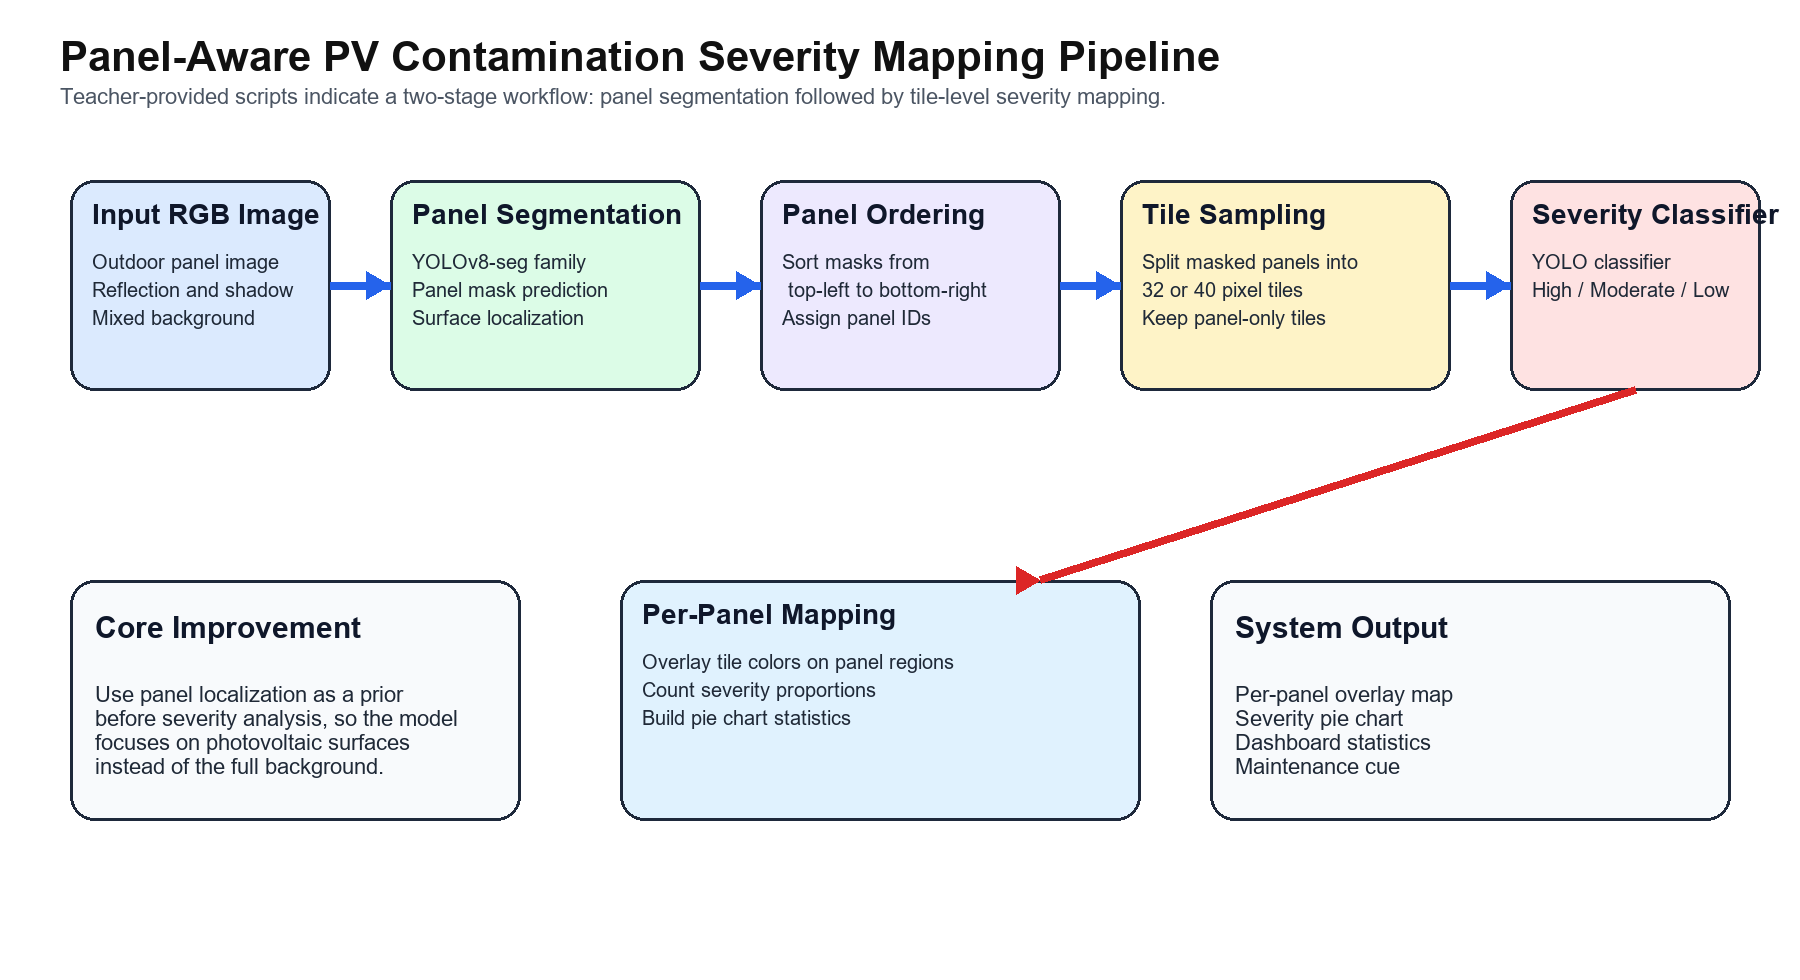
\includegraphics[width=\columnwidth]{assets/framework_overview.png}}
\caption{Panel-aware contamination severity mapping framework derived from the teacher-provided scripts and the current reproducible pipeline.}
\label{fig_framework}
\end{figure}

\subsection{Panel-Aware Localization Prior}
The main methodological choice in this work is to insert panel localization before severity analysis. This is the single explicit improvement point claimed in the draft. Instead of classifying the full image, the framework first restricts the analysis region to predicted PV surfaces. This reduces interference from roof edges, ground texture, metal frames, and other non-panel structures.

The current reproducible segmentation baseline uses the YOLOv8 segmentation family. The teacher-provided training script targets YOLOv8m-seg, while the stable draft baseline reported in this paper uses a lightweight \texttt{yolov8n-seg} reproduction because the available environment is CPU-only. The method itself is independent of a specific scale variant.

\subsection{Tile-Level Severity Mapping}
After panel masking, the image is divided into small tiles. The teacher-provided inference script uses a tile size of 32 pixels for smaller images and 40 pixels for larger images. Only tiles that overlap with a predicted panel region are classified. Let the tile prediction for panel $k$ be $c_{k,i} \in \{\text{High}, \text{Moderate}, \text{Low}\}$. The panel-level severity histogram is
\begin{equation}
h_k = [n_k^{H}, n_k^{M}, n_k^{L}],
\end{equation}
where $n_k^{H}$, $n_k^{M}$, and $n_k^{L}$ are the numbers of tiles assigned to the three severity levels. The normalized ratio
\begin{equation}
r_k = \frac{h_k}{n_k^{H} + n_k^{M} + n_k^{L}}
\end{equation}
is used to generate a pie chart and to identify the dominant severity level for panel $k$.

\subsection{Training and Evaluation Strategy}
The current draft reports reproducible stage-wise baselines rather than a final camera-ready comparison. The segmentation stage is evaluated by IoU, Dice, pixel-level precision, pixel-level recall, and mask mAP. The severity classification stage is evaluated by accuracy, Macro-Precision, Macro-Recall, Macro-F1, and the confusion matrix. This metric selection follows the review logic for image segmentation and classification papers and avoids mixing unsupported detection metrics with the present labels.

\section{Experiments}
\subsection{Dataset and Implementation Details}
The available annotated data naturally define a two-stage task. The first dataset is for panel segmentation and contains \SegTrain{} training images, \SegVal{} validation images, and \SegTest{} test images. These RGB images span a large resolution range, from $163 \times 143$ to $2048 \times 2048$ pixels in the training split. The labels are binary panel masks with a single class, namely PV surface.

The second dataset is for tile-level severity classification and contains \ClsTotal{} small image patches. The original data release provided train/test folders only. To obtain a stable validation protocol, we randomly sampled 10\% of the provided training tiles with seed 42, resulting in \ClsTrain{} training tiles, \ClsVal{} validation tiles, and \ClsTest{} test tiles. The three classes are High, Moderate, and Low contamination severity. The raw tile sizes range from $25 \times 25$ to $52 \times 52$ pixels.

The current reproducible baseline was executed in a CPU-only environment with Ultralytics 8.4.21. The segmentation baseline uses \texttt{yolov8n-seg} with 320-pixel input resolution and batch size 2. The severity classifier uses \texttt{yolo11n-cls} with 224-pixel input resolution and batch size 32. These settings are sufficient to establish a stable minimum baseline and a working end-to-end pipeline, but stronger same-family comparisons should be added before final submission.

\begin{table}[htbp]
\caption{Dataset definition used in the current draft.}
\label{tab_dataset}
\centering
\begin{tabular}{lcc}
\toprule
Stage & Split & Size \\
\midrule
Panel segmentation & train / val / test & \SegTrain{} / \SegVal{} / \SegTest{} \\
Severity classification & train / val / test & \ClsTrain{} / \ClsVal{} / \ClsTest{} \\
Severity classes & tile labels & High / Moderate / Low \\
\bottomrule
\end{tabular}
\end{table}

\subsection{Stage-Wise Baseline Results}
Table~\ref{tab_stage_results} reports the current real metrics. For panel segmentation, the mean IoU reaches \SegIoU{}\% and the mean Dice score reaches \SegDice{}\%. For severity classification, the top-1 accuracy is \ClsAcc{}\% and the Macro-F1 is \ClsMacroF{}\%. These numbers show that both stages are already usable as a minimum baseline.

\begin{table}[htbp]
\caption{Current reproducible stage-wise baseline results.}
\label{tab_stage_results}
\centering
\begin{tabular}{lcccc}
\toprule
Stage & Precision (\%) & Recall (\%) & Main score 1 & Main score 2 \\
\midrule
Segmentation & \SegPrecision{} & \SegRecall{} & IoU \SegIoU{} & Dice \SegDice{} \\
Severity classification & \ClsMacroP{} & \ClsMacroR{} & Acc. \ClsAcc{} & Macro-F1 \ClsMacroF{} \\
\bottomrule
\end{tabular}
\end{table}

The Ultralytics validation output also reports mask mAP@0.5 = \SegMapFifty{}\% and mask mAP@0.5:0.95 = \SegMapNinetyFive{}\% for the segmentation stage. The classification confusion matrix indicates that the dominant confusion pair is Moderate versus High. In the current test set, 78 Moderate samples are predicted as High, while the Low class remains comparatively stable.

\begin{table}[htbp]
\caption{Per-class classification performance on the current test set.}
\label{tab_cls_perclass}
\centering
\begin{tabular}{lccc}
\toprule
Class & Precision (\%) & Recall (\%) & F1 (\%) \\
\midrule
High & 88.29 & 97.51 & 92.67 \\
Moderate & 93.37 & 85.25 & 89.12 \\
Low & 96.96 & 95.28 & 96.11 \\
\bottomrule
\end{tabular}
\end{table}

\subsection{Visualization and Error Analysis}
Figure~\ref{fig_examples} shows representative images from the two datasets, and Fig.~\ref{fig_qualitative} summarizes the current visual evidence. The segmentation preview confirms that the model can localize PV surfaces in multi-panel scenes, while the normalized confusion matrix makes the class-level error pattern visible.

\begin{figure}[htbp]
\centerline{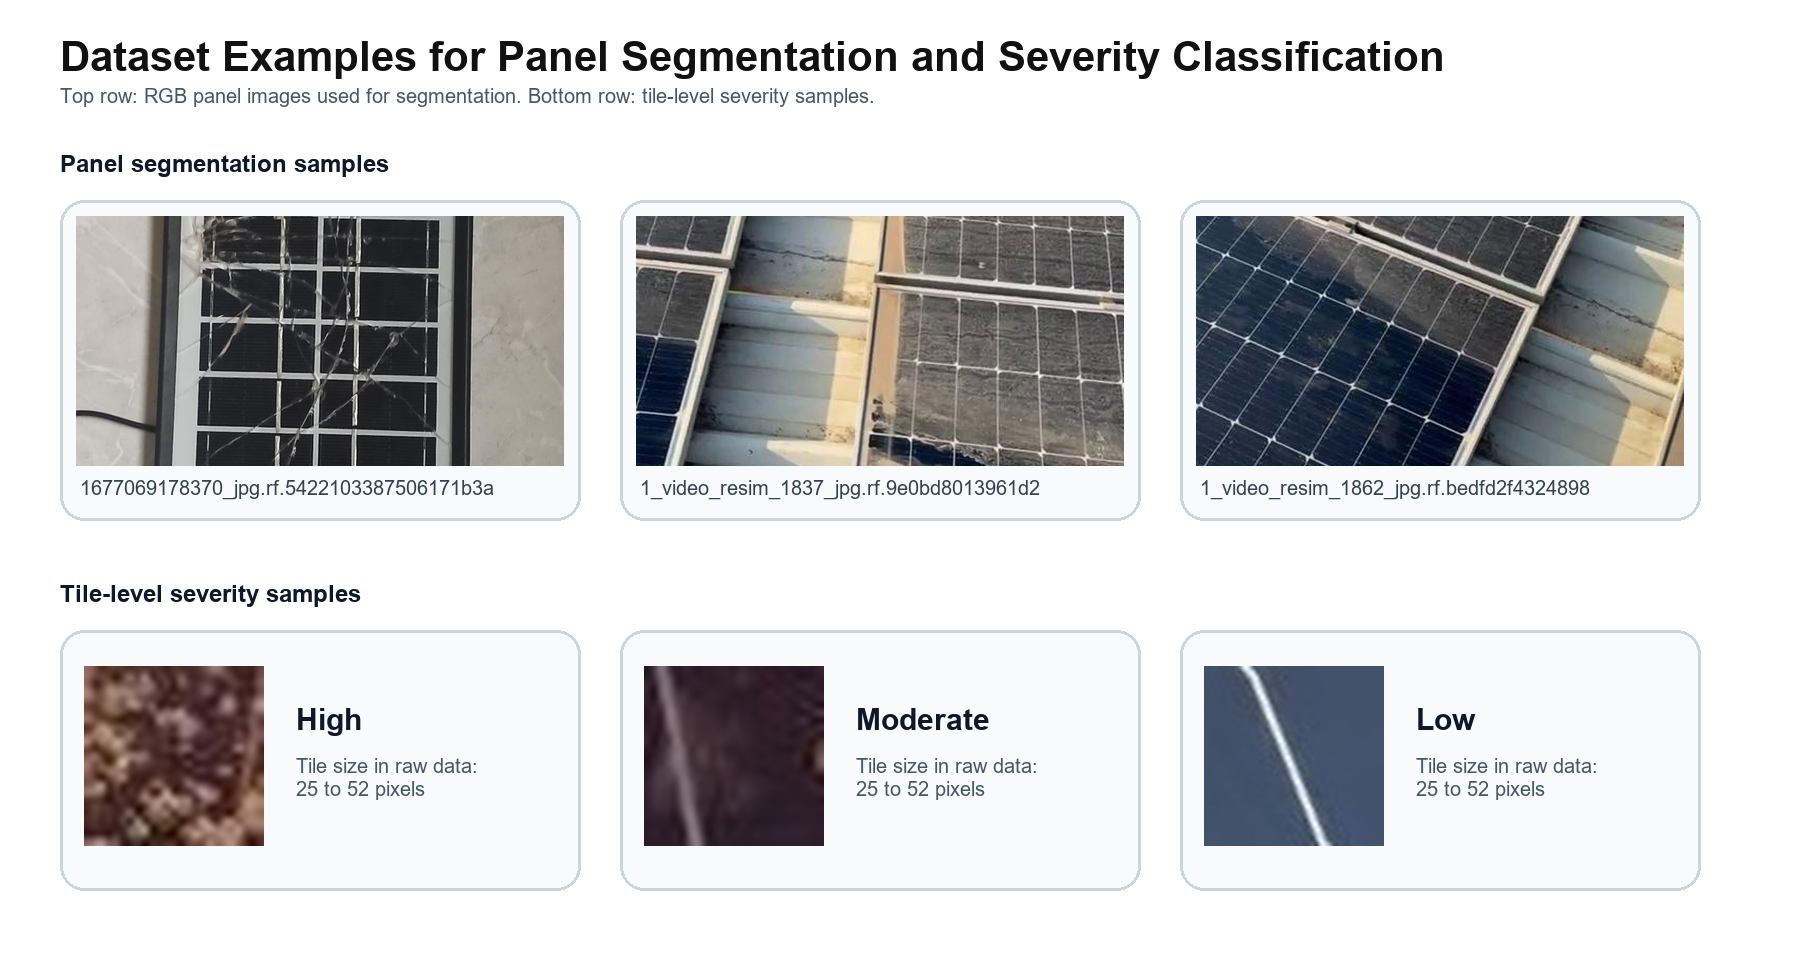
\includegraphics[width=\columnwidth]{assets/pv_examples.png}}
\caption{Representative examples from the panel segmentation dataset and the tile-level severity classification dataset.}
\label{fig_examples}
\end{figure}

\begin{figure}[htbp]
\centerline{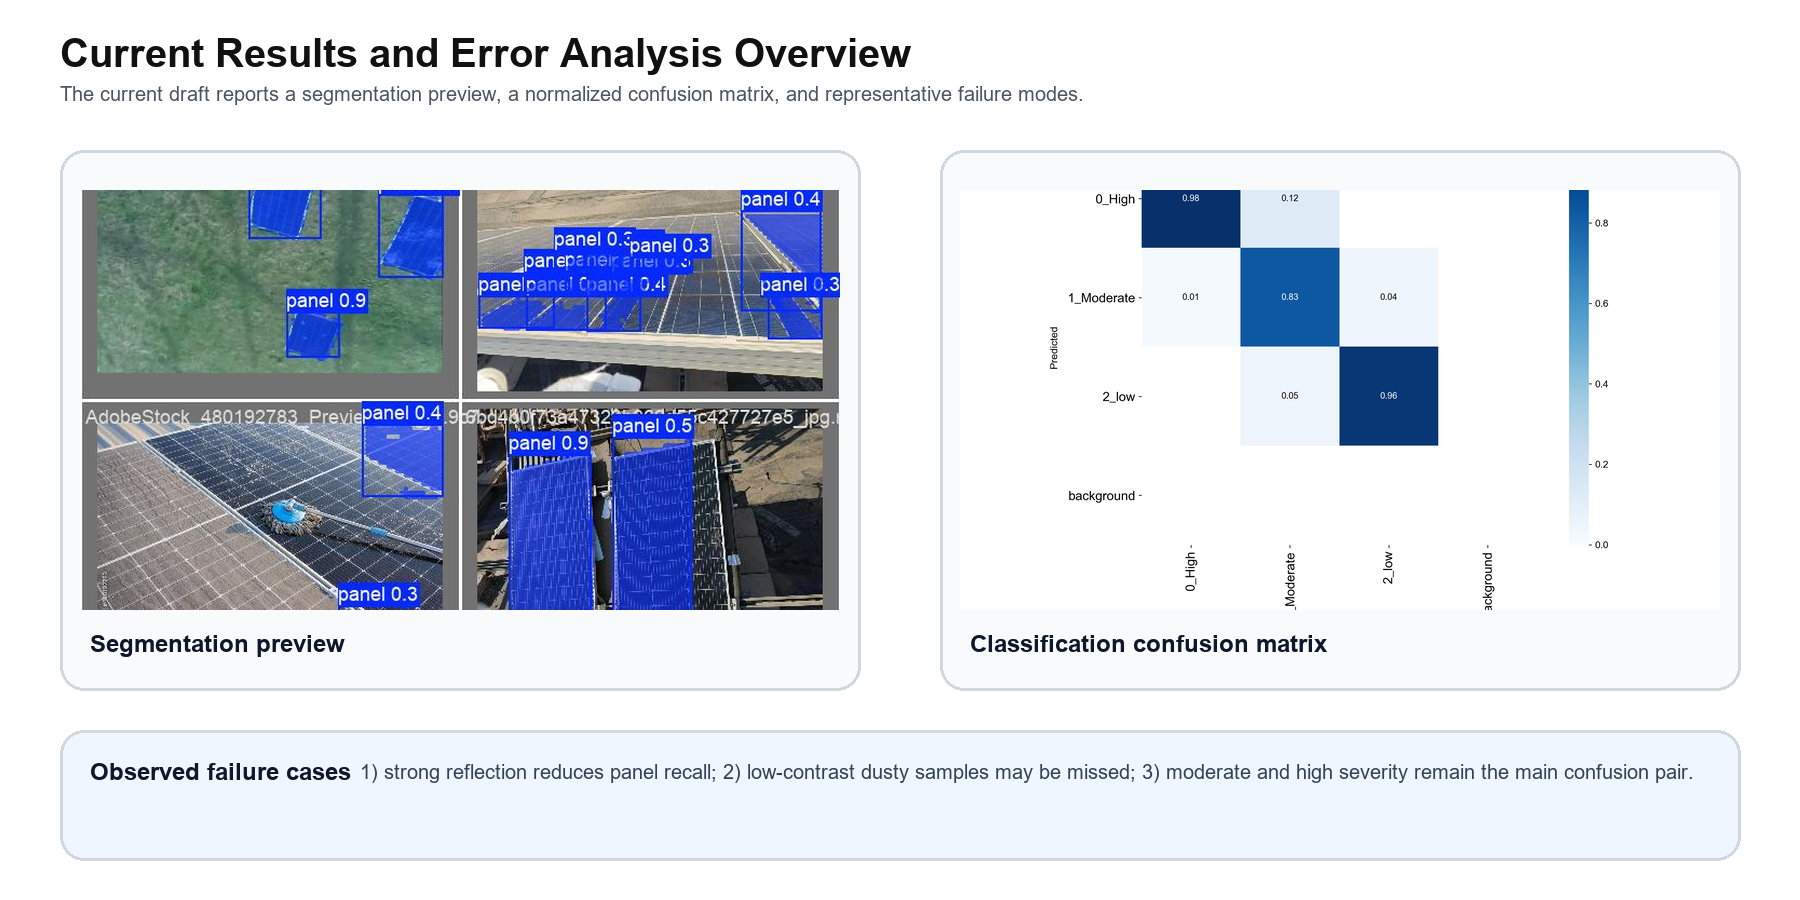
\includegraphics[width=\columnwidth]{assets/qualitative_results.png}}
\caption{Current qualitative and error-analysis overview, including segmentation preview and the normalized confusion matrix.}
\label{fig_qualitative}
\end{figure}

The observed failure modes can be grouped into three categories. First, strong reflection may suppress local panel texture and reduce segmentation recall. Second, low-contrast dusty samples can produce missed panel regions or unstable tile predictions. Third, Moderate and High severity remain the main confusion pair, which suggests that future comparisons should focus on better severity calibration rather than only higher overall accuracy. These findings already satisfy the minimum requirement for qualitative success and failure analysis in a short ICSIP-style paper.

\subsection{What Is Still Missing Before Submission}
Although the draft is now aligned with the available data and real baseline logs, two key pieces are still needed before a proper submission. First, at least two to three same-family comparison baselines should be added, for example a direct tile classifier baseline without panel prior and a larger backbone baseline. Second, a clean ablation table is still required if the final paper claims more than the current panel-aware localization prior.

\section{Conclusion}
This paper draft freezes the task as panel-aware contamination severity mapping under complex illumination. The pipeline combines panel segmentation, tile-level severity classification, and per-panel aggregation, and it already has reproducible stage-wise baselines with real metrics. More importantly, the narrative is now consistent with the teacher-provided scripts and the currently available annotations. Before submission, the remaining work is to complete acquisition metadata, same-family comparison baselines, and a final ablation table, rather than to change the task definition again.

\begin{thebibliography}{00}
\bibitem{ref_review} M. Islam, M. R. Rashel, M. T. Ahmed, A. K. M. K. Islam, and M. Tlem\c{c}ani, ``Artificial Intelligence in Photovoltaic Fault Identification and Diagnosis: A Systematic Review,'' \textit{Energies}, vol. 16, no. 21, Art. no. 7417, 2023, doi: 10.3390/en16217417.
\bibitem{ref_aerial} E. Arnaudo, G. Blanco, A. Monti, G. Bianco, C. Monaco, P. Pasquali, and F. Dominici, ``A Comparative Evaluation of Deep Learning Techniques for Photovoltaic Panel Detection From Aerial Images,'' \textit{IEEE Access}, vol. 11, pp. 47579--47594, 2023, doi: 10.1109/ACCESS.2023.3275435.
\bibitem{ref_rgbsoiling} R. Cavieres, R. Barraza, D. Estay, J. Bilbao, and P. Valdivia-Lefort, ``Automatic soiling and partial shading assessment on PV modules through RGB images analysis,'' \textit{Applied Energy}, vol. 306, Art. no. 117964, 2022, doi: 10.1016/j.apenergy.2021.117964.
\bibitem{ref_vissoiling} B. I. Evstatiev, D. T. Trifonov, K. G. Gabrovska-Evstatieva, N. P. Valov, and N. P. Mihailov, ``PV Module Soiling Detection Using Visible Spectrum Imaging and Machine Learning,'' \textit{Energies}, vol. 17, no. 20, Art. no. 5238, 2024, doi: 10.3390/en17205238.
\bibitem{ref_deepsolareye} S. Mehta, A. P. Azad, S. A. Chemmengath, V. Raykar, and S. Kalyanaraman, ``DeepSolarEye: Power Loss Prediction and Weakly Supervised Soiling Localization via Fully Convolutional Networks for Solar Panels,'' in \textit{Proc. IEEE Winter Conf. Appl. Comput. Vis.}, 2018, pp. 333--342, doi: 10.1109/WACV.2018.00043.
\bibitem{ref_uavfault} S. Jumaboev, D. Jurakuziev, and M. Lee, ``Photovoltaics Plant Fault Detection Using Deep Learning Techniques,'' \textit{Remote Sensing}, vol. 14, no. 15, Art. no. 3728, 2022, doi: 10.3390/rs14153728.
\bibitem{ref_yolo} J. Redmon, S. Divvala, R. Girshick, and A. Farhadi, ``You Only Look Once: Unified, Real-Time Object Detection,'' in \textit{Proc. IEEE Conf. Comput. Vis. Pattern Recognit.}, 2016, pp. 779--788, doi: 10.1109/CVPR.2016.91.
\bibitem{ref_ultralytics} G. Jocher \textit{et al.}, ``Ultralytics YOLO,'' GitHub repository, 2024. [Online]. Available: https://github.com/ultralytics/ultralytics
\end{thebibliography}

\end{document}
